% Options for packages loaded elsewhere
\PassOptionsToPackage{unicode}{hyperref}
\PassOptionsToPackage{hyphens}{url}
%
\documentclass[
]{article}
\usepackage{amsmath,amssymb}
\usepackage{iftex}
\ifPDFTeX
  \usepackage[T1]{fontenc}
  \usepackage[utf8]{inputenc}
  \usepackage{textcomp} % provide euro and other symbols
\else % if luatex or xetex
  \usepackage{unicode-math} % this also loads fontspec
  \defaultfontfeatures{Scale=MatchLowercase}
  \defaultfontfeatures[\rmfamily]{Ligatures=TeX,Scale=1}
\fi
\usepackage{lmodern}
\ifPDFTeX\else
  % xetex/luatex font selection
\fi
% Use upquote if available, for straight quotes in verbatim environments
\IfFileExists{upquote.sty}{\usepackage{upquote}}{}
\IfFileExists{microtype.sty}{% use microtype if available
  \usepackage[]{microtype}
  \UseMicrotypeSet[protrusion]{basicmath} % disable protrusion for tt fonts
}{}
\makeatletter
\@ifundefined{KOMAClassName}{% if non-KOMA class
  \IfFileExists{parskip.sty}{%
    \usepackage{parskip}
  }{% else
    \setlength{\parindent}{0pt}
    \setlength{\parskip}{6pt plus 2pt minus 1pt}}
}{% if KOMA class
  \KOMAoptions{parskip=half}}
\makeatother
\usepackage{xcolor}
\usepackage[margin=1in]{geometry}
\usepackage{color}
\usepackage{fancyvrb}
\newcommand{\VerbBar}{|}
\newcommand{\VERB}{\Verb[commandchars=\\\{\}]}
\DefineVerbatimEnvironment{Highlighting}{Verbatim}{commandchars=\\\{\}}
% Add ',fontsize=\small' for more characters per line
\usepackage{framed}
\definecolor{shadecolor}{RGB}{248,248,248}
\newenvironment{Shaded}{\begin{snugshade}}{\end{snugshade}}
\newcommand{\AlertTok}[1]{\textcolor[rgb]{0.94,0.16,0.16}{#1}}
\newcommand{\AnnotationTok}[1]{\textcolor[rgb]{0.56,0.35,0.01}{\textbf{\textit{#1}}}}
\newcommand{\AttributeTok}[1]{\textcolor[rgb]{0.13,0.29,0.53}{#1}}
\newcommand{\BaseNTok}[1]{\textcolor[rgb]{0.00,0.00,0.81}{#1}}
\newcommand{\BuiltInTok}[1]{#1}
\newcommand{\CharTok}[1]{\textcolor[rgb]{0.31,0.60,0.02}{#1}}
\newcommand{\CommentTok}[1]{\textcolor[rgb]{0.56,0.35,0.01}{\textit{#1}}}
\newcommand{\CommentVarTok}[1]{\textcolor[rgb]{0.56,0.35,0.01}{\textbf{\textit{#1}}}}
\newcommand{\ConstantTok}[1]{\textcolor[rgb]{0.56,0.35,0.01}{#1}}
\newcommand{\ControlFlowTok}[1]{\textcolor[rgb]{0.13,0.29,0.53}{\textbf{#1}}}
\newcommand{\DataTypeTok}[1]{\textcolor[rgb]{0.13,0.29,0.53}{#1}}
\newcommand{\DecValTok}[1]{\textcolor[rgb]{0.00,0.00,0.81}{#1}}
\newcommand{\DocumentationTok}[1]{\textcolor[rgb]{0.56,0.35,0.01}{\textbf{\textit{#1}}}}
\newcommand{\ErrorTok}[1]{\textcolor[rgb]{0.64,0.00,0.00}{\textbf{#1}}}
\newcommand{\ExtensionTok}[1]{#1}
\newcommand{\FloatTok}[1]{\textcolor[rgb]{0.00,0.00,0.81}{#1}}
\newcommand{\FunctionTok}[1]{\textcolor[rgb]{0.13,0.29,0.53}{\textbf{#1}}}
\newcommand{\ImportTok}[1]{#1}
\newcommand{\InformationTok}[1]{\textcolor[rgb]{0.56,0.35,0.01}{\textbf{\textit{#1}}}}
\newcommand{\KeywordTok}[1]{\textcolor[rgb]{0.13,0.29,0.53}{\textbf{#1}}}
\newcommand{\NormalTok}[1]{#1}
\newcommand{\OperatorTok}[1]{\textcolor[rgb]{0.81,0.36,0.00}{\textbf{#1}}}
\newcommand{\OtherTok}[1]{\textcolor[rgb]{0.56,0.35,0.01}{#1}}
\newcommand{\PreprocessorTok}[1]{\textcolor[rgb]{0.56,0.35,0.01}{\textit{#1}}}
\newcommand{\RegionMarkerTok}[1]{#1}
\newcommand{\SpecialCharTok}[1]{\textcolor[rgb]{0.81,0.36,0.00}{\textbf{#1}}}
\newcommand{\SpecialStringTok}[1]{\textcolor[rgb]{0.31,0.60,0.02}{#1}}
\newcommand{\StringTok}[1]{\textcolor[rgb]{0.31,0.60,0.02}{#1}}
\newcommand{\VariableTok}[1]{\textcolor[rgb]{0.00,0.00,0.00}{#1}}
\newcommand{\VerbatimStringTok}[1]{\textcolor[rgb]{0.31,0.60,0.02}{#1}}
\newcommand{\WarningTok}[1]{\textcolor[rgb]{0.56,0.35,0.01}{\textbf{\textit{#1}}}}
\usepackage{longtable,booktabs,array}
\usepackage{calc} % for calculating minipage widths
% Correct order of tables after \paragraph or \subparagraph
\usepackage{etoolbox}
\makeatletter
\patchcmd\longtable{\par}{\if@noskipsec\mbox{}\fi\par}{}{}
\makeatother
% Allow footnotes in longtable head/foot
\IfFileExists{footnotehyper.sty}{\usepackage{footnotehyper}}{\usepackage{footnote}}
\makesavenoteenv{longtable}
\usepackage{graphicx}
\makeatletter
\def\maxwidth{\ifdim\Gin@nat@width>\linewidth\linewidth\else\Gin@nat@width\fi}
\def\maxheight{\ifdim\Gin@nat@height>\textheight\textheight\else\Gin@nat@height\fi}
\makeatother
% Scale images if necessary, so that they will not overflow the page
% margins by default, and it is still possible to overwrite the defaults
% using explicit options in \includegraphics[width, height, ...]{}
\setkeys{Gin}{width=\maxwidth,height=\maxheight,keepaspectratio}
% Set default figure placement to htbp
\makeatletter
\def\fps@figure{htbp}
\makeatother
\setlength{\emergencystretch}{3em} % prevent overfull lines
\providecommand{\tightlist}{%
  \setlength{\itemsep}{0pt}\setlength{\parskip}{0pt}}
\setcounter{secnumdepth}{-\maxdimen} % remove section numbering
\ifLuaTeX
  \usepackage{selnolig}  % disable illegal ligatures
\fi
\IfFileExists{bookmark.sty}{\usepackage{bookmark}}{\usepackage{hyperref}}
\IfFileExists{xurl.sty}{\usepackage{xurl}}{} % add URL line breaks if available
\urlstyle{same}
\hypersetup{
  pdftitle={rtpcr: a package for statistical analysis of real-time PCR data in R},
  pdfauthor={Ghader Mirzaghaderi},
  hidelinks,
  pdfcreator={LaTeX via pandoc}}

\title{rtpcr: a package for statistical analysis of real-time PCR data
in R}
\author{Ghader Mirzaghaderi}
\date{}

\begin{document}
\maketitle

{
\setcounter{tocdepth}{2}
\tableofcontents
}
\hypertarget{overview}{%
\section{Overview}\label{overview}}

Real-time polymerase chain reaction (real-time PCR), is widely used in
biological research. Various analysis methods are employed on the
real-time PCR data to measure the mRNA levels under different
experimental conditions. `rtpcr' package was developed for amplification
efficiency calculation and statistical analysis of real-time PCR data in
R. By accounting for up to two reference genes and amplification
efficiency values, a general calculation methodology described by Ganger
et al.~(2017), matching both Livak and Schmittgen (2001) and Pfaffl et
al.~(2002) methods was used. Based on the experimental conditions, the
functions of the `rtpcr' package use a t-test (for experiments with a
two-level factor) or analysis of variance (for cases where more than two
levels or factors or a blocking factor exist) to calculate the fold
change (FC) or relative expression (RE). The functions further provide
standard deviations and confidence limits for means, apply statistical
mean comparisons and present letter mean grouping. To facilitate
function application, different data sets were used as examples and the
outputs were explained. An outstanding feature of `rtpcr' package is
providing publication-ready bar plots with various controlling arguments
for experiments with up to three different factors.

\hypertarget{calculation-methods}{%
\section{Calculation methods}\label{calculation-methods}}

The basic method for expression estimation of a gene between conditions
relies on the calculation of fold differences by means of the PCR
amplification efficiency (E) and the threshold cycle (syn. crossing
point or Ct). Among the various approaches developed for data analysis
in real-time PCR, the Livak approach, also known as the
\(2^{-\Delta\Delta C_t}\) method, stands out for its simplicity and
widespread use where the fold change (FC) exoression
(\(2^{-\Delta\Delta C_t}\)) in Treatment (Tr) compared to Control (Co)
condition is calculated according to equation:

\[\begin{align*}
\text{Fold change} & = 2^{-\Delta\Delta C_t} \\
& = \frac{2^{-(C_{t_{\text{target}}}-C_{t_{\text{ref}}})_{Tr}}}
{2^{-(C_{t_{\text{target}}}-C_{t_{\text{ref}}})_{Co}}} \\ 
& =2^{-[(C_{t_{\text{target}}}-C_{t_{\text{ref}}})_{\text{Tr}}-
{(C_{t_{\text{target}}}-C_{t_{\text{ref}}})}_{\text{Co}}]} \\ 
& = 2^{-[{(\Delta C_t)_{Tr} - (\Delta C_t)_{Co}}]}
\end{align*}\]

Here, \(\Delta C_t\) is the difference between two Ct values
(e.g.~Cttarget−Ctref) and target and ref are target gene and reference
genes, respectively. This method assumes that both the target and
reference genes are amplified with efficiencies close to 100\%, allowing
for the relative quantification of gene expression levels This method
assumes that both the target and reference genes are amplified with
efficiencies close to 100\%, allowing for the relative quantification of
gene expression levels.

On the other hand, the Pfaffl method offers a more flexible approach by
accounting for differences in amplification efficiencies between the
target and reference genes. This method adjusts the calculated
expression ratio by incorporating the specific amplification
efficiencies, thus providing a more accurate representation of the
relative gene expression levels.

\[\text{Fold change} = \frac{E^{-(C_{t_{\text{Tr}}}-C_{t_{\text{Co}}})_{target}}}
{E^{-(C_{t_{\text{Tr}}}-C_{t_{\text{Co}}})_{ref}}}\]

\hypertarget{a-generalized-calculation-method}{%
\section{A generalized calculation
method}\label{a-generalized-calculation-method}}

The rtpcr package was developed for the R environment in the major
operating systems. The packager functions are mainly based on the
calculation of efficiency-weighted \(\Delta C_t\) (\(w\Delta C_t\))
values from target and reference gene Ct (equation 3). \(w\Delta C_t\)
values are weighted for the amplification efficiencies as described by
Ganger et al.~(2017):

\[w\Delta Ct =\log_{10}(E_{target}).Ct_{target}-\log_{10}(E_{ref}).Ct_{ref}\]

From the mean wΔCt values over biological replicates, relative
expression (RE) of a target gene can be calculated for each condition
according to the equation

\[\text{Relative Expression} = 10^{-\overline{w\Delta Ct}}\] When there
are only a two conditional factor (e.g.~with treatment and control
levels), or there is one multi-level factor that one of them is
concidered as control, average fold change (FC) expression of target
gene can be calculated according to:

\[\text{Fold Change}=10^{-(\overline{w\Delta Ct}_{\text{Tr}}-{\overline{w\Delta Ct}_{\text{Co}}})}\]

in rtpcr package, `qpcrTTEST', `qpcrTTESTplot' finctions calcualtes FC
for multi-genes-two conditional cases and `qpcrANCOVA' represents FC for
single-gene-single factor or single-gene-multi factorial experiments. If
wDCt values is calculated from the E valuses, these calculations match
the formula of Pfaffl while if 2 (complete efficiency) be used instead,
the result match the \(2^{-\Delta\Delta C_t}\) method. In any case we
called these as Fold Change in the outputs of `rtpcr'. Under factorial
experiments where the calculation of the expression of the target gene
relative to the reference gene (called Relative Expression) in each
condition is desired, `qpcrANOVA', `oneFACTORplot', `twoFACTORplot' and
`threeFACTORplot' functions were developed for ANOVA analysis, and
representing the plots from single, double or triple factor experiments,
respectively. The last three functions generate `ggplot2'-derived graphs
based on the output of the `qpcrANOVA' function. If available, the
blocking factor can laso be handled by `qpcrTTEST' and `qpcrANOVA'
functions. Here, a brief methodology is presented but detailes about the
\(w\Delta C_t\) calculations and statistical analysis are available in.
Importantly, because the relative or FC gene expression follow a
lognormal distribution, a normal distribution is expected for the
\(w\Delta C_t\) or \(w\Delta\Delta C_t\) values making it possible to
apply t-test or analysis of variance to them. Following analysis,
\(w\Delta C_t\) values are statistically compared and standard
deviations and confidence intervals is calculated, but the
transformation \(y = 10^x\) is applied in the final step in order to
report the results (i.e.~RE ratios, errors and confidence limits).

\hypertarget{installing-and-loading}{%
\section{Installing and loading}\label{installing-and-loading}}

The rtpcr package can be installed and loaded using:

\begin{Shaded}
\begin{Highlighting}[]
\FunctionTok{install.packages}\NormalTok{(}\StringTok{"rtpcr"}\NormalTok{)}
\FunctionTok{library}\NormalTok{(rtpcr)}
\end{Highlighting}
\end{Shaded}

Alternatively, the \texttt{rtpcr} with the latest changes can be
installed by running the following code in your R software:

\begin{Shaded}
\begin{Highlighting}[]
\CommentTok{\# install \textasciigrave{}rtpcr\textasciigrave{} from github (under development)}

\NormalTok{devtools}\SpecialCharTok{::}\FunctionTok{install\_github}\NormalTok{(}\StringTok{"mirzaghaderi/rtpcr"}\NormalTok{)}

\CommentTok{\# I strongly recommend to install the package with the vignette as it contains information about how to use the \textquotesingle{}rtpcr\textquotesingle{} package. Through the following code, Vignette is installed as well.}

\NormalTok{devtools}\SpecialCharTok{::}\FunctionTok{install\_github}\NormalTok{(}\StringTok{"mirzaghaderi/rtpcr"}\NormalTok{, }\AttributeTok{build\_vignettes =} \ConstantTok{TRUE}\NormalTok{)}
\end{Highlighting}
\end{Shaded}

\hypertarget{data-structure-and-column-arrangement}{%
\section{Data structure and column
arrangement}\label{data-structure-and-column-arrangement}}

To use the functions, input data should be prepared in the right format
with appropriate column arrangement. The correct column arrangement is
shown in Table 1.

\emph{Table 1. Data structure and column arrangement required for
`rtpcr' package. rep: technical replicate; targetE and refE:
amplification efficiency columns for target and reference genes
respectively. targetCt and refCt: target and reference Ct columns,
respectively. factors (factor1, factor2 and/or factor3): experimental
factors.}

\begin{longtable}[]{@{}
  >{\raggedright\arraybackslash}p{(\columnwidth - 4\tabcolsep) * \real{0.2366}}
  >{\raggedright\arraybackslash}p{(\columnwidth - 4\tabcolsep) * \real{0.3871}}
  >{\raggedright\arraybackslash}p{(\columnwidth - 4\tabcolsep) * \real{0.3763}}@{}}
\toprule\noalign{}
\begin{minipage}[b]{\linewidth}\raggedright
Experiment type
\end{minipage} & \begin{minipage}[b]{\linewidth}\raggedright
Column arrangement of the input data
\end{minipage} & \begin{minipage}[b]{\linewidth}\raggedright
Example in the package
\end{minipage} \\
\midrule\noalign{}
\endhead
\bottomrule\noalign{}
\endlastfoot
Amplification efficiency & Dilutions - targetCt - refCt &
data\_efficiency \\
t-test (accepts multiple genes) & condition (put the control level
first) - gene (put reference gene(s) last.)- efficiency - Ct &
data\_ttest \\
Factorial (Up to three factors) & factor1 - rep - targetE - targetCt -
refE - refCt & data\_1factor \\
& factor1 - factor2 - rep - targetE - targetCt - refE - refCt &
data\_2factor \\
& factor1 - factor2 - factor3 - rep - targetE - targetCt - refE - refCt
& data\_3factor\_b \\
Factorial with blocking & factor1 - block - rep - targetE - targetCt -
refE - refCt & \\
& factor1 - factor2 - block - rep - targetE - targetCt - refE - refCt &
data\_2factorBlock \\
& factor1 - factor2 - factor3 - block - rep - targetE - targetCt - refE
- refCt & \\
Two reference genes & . . . . . . rep - targetE - targetCt - ref1E -
ref1Ct - ref2E - ref2Ct & \\
calculating biological replicated & . . . . . . biologicalRep -
techcicalRep - Etarget - targetCt - Eref - refCt & data\_withTechRep \\
& . . . . . . biologicalRep - techcicalRep - Etarget - targetCt - ref1E
- ref1Ct - ref2E - ref2Ct & \\
\end{longtable}

\hypertarget{functions-usage}{%
\section{functions usage}\label{functions-usage}}

To simplify `rtpcr' usage, examples for using the functions are
presented below.

\emph{Table 2. Functions and examples for using them.} \textbar{}
function \textbar{} Analysis \textbar{} Example (see package help for
the more arguments) \textbar{}
\textbar:---------------------\textbar:-----------------------------------\textbar:----------------------------------\textbar{}
\textbar{} efficiency \textbar{} Efficiency, standard curves and related
statistics \textbar{} efficiency(data\_efficiency) \textbar{} \textbar{}
meanTech \textbar{} Calculating the mean of technical replicates
\textbar{} meanTech(data\_withTechRep, groups = 1:4) \textbar{}
\textbar{} qpcrANCOVA \textbar{} FC and bar plot of the target gene (one
or multi-factorial experiments) \textbar{} qpcrANCOVA(data\_1factor,
numberOfrefGenes = 1, mainFactor.column = 1, mainFactor.level.order =
c(``L1'', ``L2'', ``L3'') \textbar{} \textbar{} oneFACTORplot \textbar{}
Bar plot of the relative gene expression from a one-factor experiment
\textbar{} out \textless- qpcrANOVA(data\_1factor, numberOfrefGenes =
1)\(Result; oneFACTORplot(out) |  | qpcrANOVA | Analysis of Variance of the qpcr data | qpcrANOVA(data_3factor_a, numberOfrefGenes = 1, p.adj = "none")|  | qpcrTTEST | Computing the average fold change and related statistics | qpcrTTEST(data_ttest, numberOfrefGenes = 1, paired = FALSE, var.equal = TRUE) |  | qpcrTTESTplot | Bar plot of the average fold change of the target genes | qpcrTTESTplot(data_ttest, numberOfrefGenes = 1, order = c("C2H2-01", "C2H2-12", "C2H2-26")) |  | threeFACTORplot | Bar plot of the relative gene expression from a three-factor experiment | res <- qpcrANOVA(data_3factor_b, numberOfrefGenes = 1)\)Result;
threeFACTORplot(res, arrangement = c(3, 1, 2)) \textbar{} \textbar{}
twoFACTORplot \textbar{} Bar plot of the relative gene expression from a
two-factor experiment \textbar{} res \textless- qpcrANOVA(data\_2factor,
numberOfrefGenes = 1)\$Result; twoFACTORplot(res, x.axis.factor =
Genotype, group.factor = Drought) \textbar{}

\emph{see package help for more arguments including the number of
reference genes, levels arrangement, blocking, and arguments for
adjusting the bar plots.}

\hypertarget{amplification-efficiency-data-analysis}{%
\section{Amplification efficiency data
analysis}\label{amplification-efficiency-data-analysis}}

\hypertarget{sample-data-of-amplification-efficiency}{%
\subsection{Sample data of amplification
efficiency}\label{sample-data-of-amplification-efficiency}}

To calculate the amplification efficiencies of a target and a reference
gene, a data frame should be prepared with 3 columns of dilutions,
target gene Ct values, and reference gene Ct values, respectively, as
shown below.

\begin{Shaded}
\begin{Highlighting}[]
\NormalTok{data\_efficiency}
\end{Highlighting}
\end{Shaded}

\begin{verbatim}
##    dilutions  C2H2.26    GAPDH
## 1       1.00 25.57823 22.60794
## 2       1.00 25.53636 22.68348
## 3       1.00 25.50280 22.62602
## 4       0.50 26.70615 23.67162
## 5       0.50 26.72720 23.64855
## 6       0.50 26.86921 23.70494
## 7       0.20 28.16874 25.11064
## 8       0.20 28.06759 25.11985
## 9       0.20 28.10531 25.10976
## 10      0.10 29.19743 26.16919
## 11      0.10 29.49406 26.15119
## 12      0.10 29.07117 26.15019
## 13      0.05 30.16878 27.11533
## 14      0.05 30.14193 27.13934
## 15      0.05 30.11671 27.16338
## 16      0.02 31.34969 28.52016
## 17      0.02 31.35254 28.57228
## 18      0.02 31.34804 28.53100
## 19      0.01 32.55013 29.49048
## 20      0.01 32.45329 29.48433
## 21      0.01 32.27515 29.26234
\end{verbatim}

\hypertarget{calculating-amplification-efficiency}{%
\subsection{Calculating amplification
efficiency}\label{calculating-amplification-efficiency}}

The following \texttt{efficiency} function calculates the amplification
efficiency of a target and a reference gene and presents the related
standard curves along with the Slope, Efficiency, and R2 statistics. The
function also compares the slopes of the two standard curves. For this,
a regression line is fitted using the \(\Delta C_t\) values. If
\(2^{-\Delta\Delta C_t}\) method is intended, the slope should not
exceed 0.2!

\begin{Shaded}
\begin{Highlighting}[]
\FunctionTok{efficiency}\NormalTok{(data\_efficiency)}
\end{Highlighting}
\end{Shaded}

\begin{verbatim}
## $plot
\end{verbatim}

\begin{figure}

{\centering 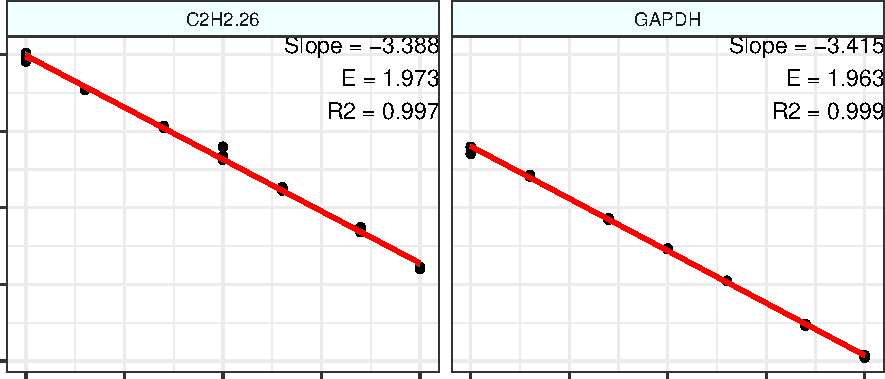
\includegraphics{vignette_files/figure-latex/unnamed-chunk-4-1} 

}

\caption{Standard curve and the amplification efficiency analysis of target and reference genes. A sample data arrangement that is required as input for the calculation of amplification efficiency by the efficiency function.}\label{fig:unnamed-chunk-4}
\end{figure}

\begin{verbatim}
## 
## $Efficiency_Analysis_Results
##      Gene  Slope     E    R2
## 1 C2H2.26 -3.388 1.973 0.997
## 2   GAPDH -3.415 1.963 0.999
## 
## $Slope_of_differences
## [1] 0.0264574
\end{verbatim}

\hypertarget{expression-data-analysis}{%
\section{Expression data analysis}\label{expression-data-analysis}}

\hypertarget{target-genes-in-two-conditions-t-test}{%
\subsection{Target genes in two conditions
(t-test)}\label{target-genes-in-two-conditions-t-test}}

\hypertarget{example-data}{%
\subsubsection{Example data}\label{example-data}}

When a target gene is assessed under two different conditions (for
example Control and treatment), it is possible to calculate the average
fold change expression i.e.~\(2^{-\Delta \Delta C_t}\) of the target
gene in treatment relative to control conditions. For this, the data
should be prepared according to the following data set consisting of 4
columns belonging to condition levels, E (efficiency), genes and Ct
values, respectively. Each Ct value is the mean of technical replicates.
Complete amplification efficiencies of 2 have been assumed here for all
wells but the calculated efficiencies can be used instead.

\begin{Shaded}
\begin{Highlighting}[]
\NormalTok{data\_ttest}
\end{Highlighting}
\end{Shaded}

\begin{verbatim}
##    Condition    Gene E    Ct
## 1    control C2H2-26 2 31.26
## 2    control C2H2-26 2 31.01
## 3    control C2H2-26 2 30.97
## 4  treatment C2H2-26 2 32.65
## 5  treatment C2H2-26 2 32.03
## 6  treatment C2H2-26 2 32.40
## 7    control C2H2-01 2 31.06
## 8    control C2H2-01 2 30.41
## 9    control C2H2-01 2 30.97
## 10 treatment C2H2-01 2 28.85
## 11 treatment C2H2-01 2 28.93
## 12 treatment C2H2-01 2 28.90
## 13   control C2H2-12 2 28.50
## 14   control C2H2-12 2 28.40
## 15   control C2H2-12 2 28.80
## 16 treatment C2H2-12 2 27.90
## 17 treatment C2H2-12 2 28.00
## 18 treatment C2H2-12 2 27.90
## 19   control     ref 2 28.87
## 20   control     ref 2 28.42
## 21   control     ref 2 28.53
## 22 treatment     ref 2 28.31
## 23 treatment     ref 2 29.14
## 24 treatment     ref 2 28.63
\end{verbatim}

\hypertarget{data-analysis-under-two-conditions}{%
\subsubsection{Data analysis under two
conditions}\label{data-analysis-under-two-conditions}}

Here, the above data set was used for the Fold Change expression
analysis of the target genes using the \texttt{qpcrTTEST} function. This
function performs a t-test-based analysis of any number of genes that
have been evaluated under control and treatment conditions. The analysis
can be done for unpaired or paired conditions. The output is a table of
target gene names, fold changes confidence limits, and the t.test
derived p-values. The \texttt{qpcrTTEST} function includes the
\texttt{var.equal} argument. When set to \texttt{FALSE}, \texttt{t.test}
is performed under the unequal variances hypothesis.

\begin{Shaded}
\begin{Highlighting}[]
\FunctionTok{qpcrTTEST}\NormalTok{(data\_ttest, }
          \AttributeTok{numberOfrefGenes =} \DecValTok{1}\NormalTok{,}
          \AttributeTok{paired =}\NormalTok{ F, }
          \AttributeTok{var.equal =}\NormalTok{ T)}
\end{Highlighting}
\end{Shaded}

\begin{verbatim}
## $Raw_data
##    Var2       wDCt
## 1     1  0.7194617
## 2     1  0.7796677
## 3     1  0.7345132
## 4     1  1.3064702
## 5     1  0.8699767
## 6     1  1.1348831
## 7     2  0.6592557
## 8     2  0.5990497
## 9     2  0.7345132
## 10    2  0.1625562
## 11    2 -0.0632163
## 12    2  0.0812781
## 13    3 -0.1113811
## 14    3 -0.0060206
## 15    3  0.0812781
## 16    3 -0.1234223
## 17    3 -0.3431742
## 18    3 -0.2197519
## 
## $Result
##      Gene     dif     FC    LCL    UCL pvalue
## 1 C2H2-26  0.3592 0.4373 0.1926 0.9927 0.0488
## 2 C2H2-01 -0.6041 4.0185 2.4598 6.5649 0.0014
## 3 C2H2-12 -0.2167 1.6472 0.9595 2.8279 0.0624
\end{verbatim}

\hypertarget{generating-plot}{%
\subsubsection{Generating plot}\label{generating-plot}}

The \texttt{qpcrTTESTplot} function generates a bar plot of Fold Changes
and confidence intervals for the target genes. the
\texttt{qpcrTTESTplot} function accepts any gene name and any
replicates. The \texttt{qpcrTTESTplot} function automatically puts
appropriate signs of **, * on top of the plot columns based on the
output p-values.

\begin{Shaded}
\begin{Highlighting}[]
\CommentTok{\# Producing the plot}
\NormalTok{t1 }\OtherTok{\textless{}{-}} \FunctionTok{qpcrTTESTplot}\NormalTok{(data\_ttest,}
              \AttributeTok{numberOfrefGenes =} \DecValTok{1}\NormalTok{,}
              \AttributeTok{fontsizePvalue =} \DecValTok{4}\NormalTok{)}

\CommentTok{\# Producing the plot: specifying gene order}
\NormalTok{t2 }\OtherTok{\textless{}{-}} \FunctionTok{qpcrTTESTplot}\NormalTok{(data\_ttest,}
              \AttributeTok{numberOfrefGenes =} \DecValTok{1}\NormalTok{,}
              \AttributeTok{order =} \FunctionTok{c}\NormalTok{(}\StringTok{"C2H2{-}01"}\NormalTok{, }\StringTok{"C2H2{-}12"}\NormalTok{, }\StringTok{"C2H2{-}26"}\NormalTok{),}
              \AttributeTok{paired =} \ConstantTok{FALSE}\NormalTok{,}
              \AttributeTok{var.equal =} \ConstantTok{TRUE}\NormalTok{,}
              \AttributeTok{width =} \FloatTok{0.5}\NormalTok{,}
              \AttributeTok{fill =} \StringTok{"palegreen"}\NormalTok{,}
              \AttributeTok{y.axis.adjust =} \DecValTok{0}\NormalTok{,}
              \AttributeTok{y.axis.by =} \DecValTok{2}\NormalTok{,}
              \AttributeTok{ylab =} \StringTok{"Average Fold Change (FC)"}\NormalTok{,}
              \AttributeTok{xlab =} \StringTok{"Gene"}\NormalTok{,}
              \AttributeTok{fontsizePvalue =} \DecValTok{4}\NormalTok{)}

\FunctionTok{multiplot}\NormalTok{(t1, t2, }\AttributeTok{cols =} \DecValTok{2}\NormalTok{)}
\end{Highlighting}
\end{Shaded}

\begin{verbatim}
## $plot
## 
## $plot
\end{verbatim}

\begin{Shaded}
\begin{Highlighting}[]
\FunctionTok{grid.text}\NormalTok{(}\StringTok{"A"}\NormalTok{, }\AttributeTok{x =} \FloatTok{0.02}\NormalTok{, }\AttributeTok{y =} \DecValTok{1}\NormalTok{, }\AttributeTok{just =} \FunctionTok{c}\NormalTok{(}\StringTok{"right"}\NormalTok{, }\StringTok{"top"}\NormalTok{), }\AttributeTok{gp=}\FunctionTok{gpar}\NormalTok{(}\AttributeTok{fontsize=}\DecValTok{16}\NormalTok{))}
\FunctionTok{grid.text}\NormalTok{(}\StringTok{"B"}\NormalTok{, }\AttributeTok{x =} \FloatTok{0.52}\NormalTok{, }\AttributeTok{y =} \DecValTok{1}\NormalTok{, }\AttributeTok{just =} \FunctionTok{c}\NormalTok{(}\StringTok{"right"}\NormalTok{, }\StringTok{"top"}\NormalTok{), }\AttributeTok{gp=}\FunctionTok{gpar}\NormalTok{(}\AttributeTok{fontsize=}\DecValTok{16}\NormalTok{))}
\end{Highlighting}
\end{Shaded}

\begin{figure}

{\centering 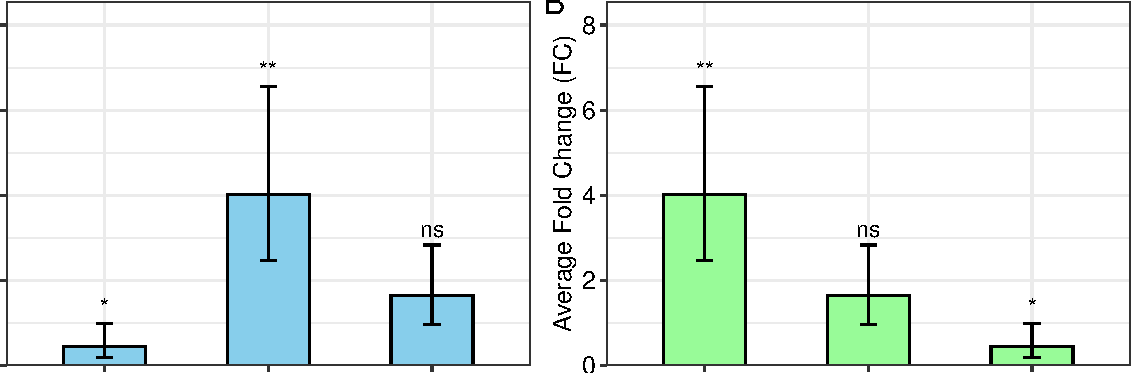
\includegraphics{vignette_files/figure-latex/unnamed-chunk-7-1} 

}

\caption{Average Fold changes of three target genes relative to the control condition computed by unpaired t-tests via ‘qpcrTTESTplot’ function.}\label{fig:unnamed-chunk-7}
\end{figure}

\hypertarget{analysis-of-covariance-ancova}{%
\subsection{Analysis of covariance
(ANCOVA)}\label{analysis-of-covariance-ancova}}

analysis of covariance (ANCOVA) is a method based on both ANOVA and
linear regression. It is basically suitable when the levels of a factor
are also affected by an uncontrolled quantitative covariate. For
example, suppose that wDCt of a target gene in a plant is affected by
temperature. The gene may also be affected by drought. since we already
know that temperature affects the target gene, we are interesting now if
the gene expression is also altered by the drought levels. We can design
an experiment to understand the gene behavior at both temperature and
drought levels at the same time. The drought is another factor (the
covariate) that may affect the expression of our gene under the levels
of the first factor i.e.~temperature. The data of such an experiment can
be analyzed by ANCOVA or even ANOVA based on a factorial experiment
using \texttt{qpcrANCOVA} function, if more than a factor exist. Bar
plot of fold changes (FCs) along with the 95\% confidence interval is
also returned by the \texttt{qpcrANCOVA} function. There is also a
function called \texttt{oneFACTORplot} which returns FC values and
related plot for a one-factor-experiment with more than two levels.

\begin{Shaded}
\begin{Highlighting}[]
\CommentTok{\# See sample data}
\NormalTok{data\_2factor}
\end{Highlighting}
\end{Shaded}

\begin{verbatim}
##    Genotype Drought Rep EPO  POCt EGAPDH GAPDHCt
## 1         R    0.00   1   2 33.30      2   31.53
## 2         R    0.00   2   2 33.39      2   31.57
## 3         R    0.00   3   2 33.34      2   31.50
## 4         R    0.25   1   2 32.73      2   31.30
## 5         R    0.25   2   2 32.46      2   32.55
## 6         R    0.25   3   2 32.60      2   31.92
## 7         R    0.50   1   2 33.48      2   33.30
## 8         R    0.50   2   2 33.27      2   33.37
## 9         R    0.50   3   2 33.32      2   33.35
## 10        S    0.00   1   2 26.85      2   26.94
## 11        S    0.00   2   2 28.17      2   27.69
## 12        S    0.00   3   2 27.99      2   27.39
## 13        S    0.25   1   2 30.41      2   28.70
## 14        S    0.25   2   2 29.49      2   28.66
## 15        S    0.25   3   2 29.98      2   28.71
## 16        S    0.50   1   2 29.03      2   30.61
## 17        S    0.50   2   2 28.73      2   30.20
## 18        S    0.50   3   2 28.83      2   30.49
\end{verbatim}

\begin{Shaded}
\begin{Highlighting}[]
\NormalTok{order }\OtherTok{\textless{}{-}} \FunctionTok{unique}\NormalTok{(data\_2factor}\SpecialCharTok{$}\NormalTok{Drought)}
\FunctionTok{qpcrANCOVA}\NormalTok{(data\_2factor, }
           \AttributeTok{numberOfrefGenes =} \DecValTok{1}\NormalTok{, }
           \AttributeTok{analysisType =} \StringTok{"ancova"}\NormalTok{,}
           \AttributeTok{mainFactor.column =} \DecValTok{2}\NormalTok{,}
           \AttributeTok{mainFactor.level.order =}\NormalTok{ order,}
           \AttributeTok{fontsizePvalue =} \DecValTok{4}\NormalTok{)}
\end{Highlighting}
\end{Shaded}

\begin{verbatim}
## $Final_data
##    Drought Genotype rep Etarget Cttarget Eref Ctref       wDCt
## 1        0        R   1       2    33.30    2 31.53  0.5328231
## 2        0        R   2       2    33.39    2 31.57  0.5478746
## 3        0        R   3       2    33.34    2 31.50  0.5538952
## 10       0        S   1       2    26.85    2 26.94 -0.0270927
## 11       0        S   2       2    28.17    2 27.69  0.1444944
## 12       0        S   3       2    27.99    2 27.39  0.1806180
## 4     0.25        R   1       2    32.73    2 31.30  0.4304729
## 5     0.25        R   2       2    32.46    2 32.55 -0.0270927
## 6     0.25        R   3       2    32.60    2 31.92  0.2047004
## 13    0.25        S   1       2    30.41    2 28.70  0.5147613
## 14    0.25        S   2       2    29.49    2 28.66  0.2498549
## 15    0.25        S   3       2    29.98    2 28.71  0.3823081
## 7      0.5        R   1       2    33.48    2 33.30  0.0541854
## 8      0.5        R   2       2    33.27    2 33.37 -0.0301030
## 9      0.5        R   3       2    33.32    2 33.35 -0.0090309
## 16     0.5        S   1       2    29.03    2 30.61 -0.4756274
## 17     0.5        S   2       2    28.73    2 30.20 -0.4425141
## 18     0.5        S   3       2    28.83    2 30.49 -0.4997098
## 
## $lm_ANOVA
## 
## Call:
## lm(formula = formula_ANOVA, data = x)
## 
## Coefficients:
##                                 (Intercept)  
##                                     0.54486  
##                      as.factor(Drought)0.25  
##                                    -0.34217  
##                       as.factor(Drought)0.5  
##                                    -0.53985  
##                        as.factor(Genotype)S  
##                                    -0.44552  
## as.factor(Drought)0.25:as.factor(Genotype)S  
##                                     0.62514  
##  as.factor(Drought)0.5:as.factor(Genotype)S  
##                                    -0.03211  
## 
## 
## $lm_ANCOVA
## 
## Call:
## lm(formula = formula_ANCOVA, data = x)
## 
## Coefficients:
##            (Intercept)    as.factor(Genotype)S  as.factor(Drought)0.25  
##                 0.4460                 -0.2478                 -0.0296  
##  as.factor(Drought)0.5  
##                -0.5559  
## 
## 
## $ANOVA_table
## Analysis of Variance Table
## 
## Response: wDCt
##                                        Df  Sum Sq Mean Sq F value    Pr(>F)    
## as.factor(Drought)                      2 1.17379 0.58690  41.394 4.117e-06 ***
## as.factor(Genotype)                     1 0.27643 0.27643  19.497 0.0008422 ***
## as.factor(Drought):as.factor(Genotype)  2 0.41190 0.20595  14.526 0.0006239 ***
## Residuals                              12 0.17014 0.01418                      
## ---
## Signif. codes:  0 '***' 0.001 '**' 0.01 '*' 0.05 '.' 0.1 ' ' 1
## 
## $ANCOVA_table
## Analysis of Variance Table
## 
## Response: wDCt
##                     Df  Sum Sq Mean Sq F value    Pr(>F)    
## as.factor(Genotype)  1 0.27643 0.27643   6.649 0.0218703 *  
## as.factor(Drought)   2 1.17379 0.58690  14.117 0.0004398 ***
## Residuals           14 0.58204 0.04157                      
## ---
## Signif. codes:  0 '***' 0.001 '**' 0.01 '*' 0.05 '.' 0.1 ' ' 1
## 
## $FC_statistics_of_the_main_factor
##                 contrast     FC pvalue sig  CI_lower CI_upper    sddiff
## 1                      0      1 1.0000     0.0000000 0.000000 0.0000000
## 2 Drought0 - Drought0.25 1.0705 0.8051  ns 0.5446459 2.104206 0.3466862
## 3  Drought0 - Drought0.5 3.5967 0.0003 *** 1.6702550 7.744999 1.3629288
## 
## $FC_Plot_of_the_main_factor_levels
\end{verbatim}

\begin{center}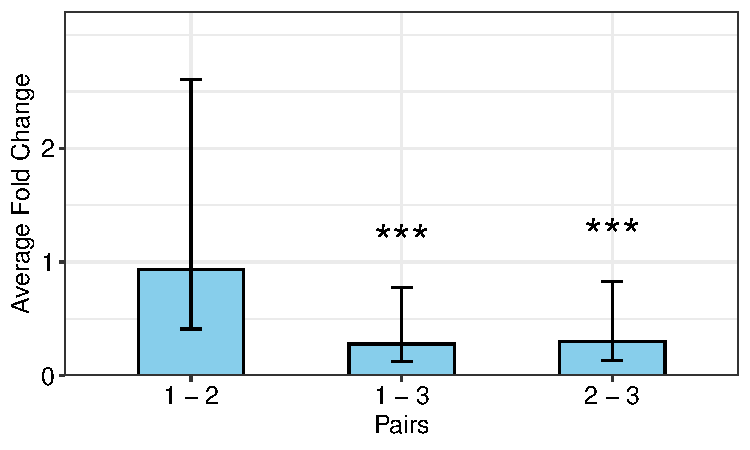
\includegraphics{vignette_files/figure-latex/unnamed-chunk-8-1} \end{center}

\hypertarget{a-target-gene-under-more-than-two-conditions-anova}{%
\subsection{A target gene under more than two conditions
(ANOVA)}\label{a-target-gene-under-more-than-two-conditions-anova}}

Analysis of variance (ANOVA) of factorial experiments in the frame of a
completely randomized design (CRD) can be done by the \texttt{qpcrANOVA}
function. ANOVA of qPCR data is suitable when there is a factor with
more than two levels, or when there is more than an experimental factor.
The input data set should be prepared as shown below. Factor columns
should be presented first followed by biological replicates and
efficiency and Ct values of target and reference genes. The example data
set below (\texttt{data\_3factor\_a}) represents amplification
efficiency and Ct values for target and reference genes under three
grouping factors (two different cultivars, three drought levels, and the
presence or absence of bacteria). The table can contain any number of
factor columns. The factor columns should be followed by five other
columns assigned to biological replicates (r), the efficiency of the
target gene, Ct values of the target gene, the efficiency of the
reference gene, and Ct values of the reference gene, respectively. Here,
the efficiency of 2 has been used for all wells, but the calculated
efficiencies can be used instead.

\begin{Shaded}
\begin{Highlighting}[]
\CommentTok{\# See a sample dataset}
\NormalTok{data\_3factor\_a}
\end{Highlighting}
\end{Shaded}

\begin{verbatim}
##    Genotype Drought SA Rep   EPO  POCt EGAPDH GAPDHCt
## 1         R    0.00 A1   1 1.839 33.30  1.918   31.53
## 2         R    0.00 A1   2 1.839 33.39  1.918   31.57
## 3         R    0.00 A1   3 1.839 33.34  1.918   31.50
## 4         R    0.00 A2   1 1.839 34.01  1.918   31.48
## 5         R    0.00 A2   2 1.839 36.82  1.918   31.44
## 6         R    0.00 A2   3 1.839 35.44  1.918   31.46
## 7         R    0.25 A1   1 1.839 32.73  1.918   31.30
## 8         R    0.25 A1   2 1.839 32.46  1.918   32.55
## 9         R    0.25 A1   3 1.839 32.60  1.918   31.92
## 10        R    0.25 A2   1 1.839 33.37  1.918   31.19
## 11        R    0.25 A2   2 1.839 33.12  1.918   31.94
## 12        R    0.25 A2   3 1.839 33.21  1.918   31.57
## 13        R    0.50 A1   1 1.839 33.48  1.918   33.30
## 14        R    0.50 A1   2 1.839 33.27  1.918   33.37
## 15        R    0.50 A1   3 1.839 33.32  1.918   33.35
## 16        R    0.50 A2   1 1.839 32.53  1.918   33.47
## 17        R    0.50 A2   2 1.839 32.61  1.918   33.26
## 18        R    0.50 A2   3 1.839 32.56  1.918   33.36
## 19        S    0.00 A1   1 1.839 26.85  1.918   26.94
## 20        S    0.00 A1   2 1.839 28.17  1.918   27.69
## 21        S    0.00 A1   3 1.839 27.99  1.918   27.39
## 22        S    0.00 A2   1 1.839 28.71  1.918   29.45
## 23        S    0.00 A2   2 1.839 29.01  1.918   29.46
## 24        S    0.00 A2   3 1.839 28.82  1.918   29.48
## 25        S    0.25 A1   1 1.839 30.41  1.918   28.70
## 26        S    0.25 A1   2 1.839 29.49  1.918   28.66
## 27        S    0.25 A1   3 1.839 29.98  1.918   28.71
## 28        S    0.25 A2   1 1.839 28.91  1.918   28.09
## 29        S    0.25 A2   2 1.839 28.60  1.918   28.65
## 30        S    0.25 A2   3 1.839 28.59  1.918   28.37
## 31        S    0.50 A1   1 1.839 29.03  1.918   30.61
## 32        S    0.50 A1   2 1.839 28.73  1.918   30.20
## 33        S    0.50 A1   3 1.839 28.83  1.918   30.49
## 34        S    0.50 A2   1 1.839 28.29  1.918   30.84
## 35        S    0.50 A2   2 1.839 28.53  1.918   30.65
## 36        S    0.50 A2   3 1.839 28.28  1.918   30.74
\end{verbatim}

The \texttt{qpcrANOVA} function performs ANOVA based on both factorial
arrangement and completely randomized design (CRD). For the latter, a
column of treatment combinations is made first as a grouping factor
followed by ANOVA. You can call the input data set along with the added
wCt and treatment combinations by \texttt{qpcrANOVA}. CRD-based analysis
is especially useful when post-hoc tests and mean comparisons/grouping
are desired for all treatment combinations. The final results along with
the ANOVA tables can be called by \texttt{qpcrANOVA}.

\hypertarget{reverse-ordering-of-the-grouping-letters}{%
\subsubsection{Reverse ordering of the grouping
letters}\label{reverse-ordering-of-the-grouping-letters}}

One may be interested in presenting the statistical mean comparison
result in the frame of grouping letters. This is rather challenging
because in the grouping output of mean comparisons (via the
\texttt{LSD.test} function of agricolae package), means are sorted into
descending order so that the largest mean, is the first in the table and
``a'' letter is assigned to it. If \texttt{LSD.test} is applied to the
wCt means, the biggest wCt mean receives ``a'' letter as expected, but
this value turns into the smallest mean after its reverse log
transformation by \(10^{-(\Delta Ct)}\). to solve this issue, I used a
function that assigns the grouping letters appropriately.

\hypertarget{output-table-of-the-analysis}{%
\subsubsection{Output table of the
analysis}\label{output-table-of-the-analysis}}

The \texttt{qpcrANOVA} function produces the main analysis output
including mean wDCt, LCL, UCL, grouping letters, and standard
deviations. The standard deviation for each mean is derived from the
back-transformed raw wDCt values from biological replicates for that
mean.

\begin{Shaded}
\begin{Highlighting}[]
\CommentTok{\# If the data include technical replicates, means of technical replicates}
\CommentTok{\# should be calculated first using meanTech function.}

\CommentTok{\# Applying ANOVA analysis}
\NormalTok{res }\OtherTok{\textless{}{-}} \FunctionTok{qpcrANOVA}\NormalTok{(data\_2factor,}
          \AttributeTok{numberOfrefGenes =} \DecValTok{1}\NormalTok{,}
          \AttributeTok{p.adj =} \StringTok{"none"}\NormalTok{)}
\NormalTok{res}\SpecialCharTok{$}\NormalTok{Result}
\end{Highlighting}
\end{Shaded}

\begin{verbatim}
##        Genotype Drought     RE    LCL    UCL letters    std
## R:0           R       0 0.2852 0.4026 0.2020       d 0.0072
## R:0.25        R    0.25 0.6271 0.8853 0.4441      bc 0.3508
## R:0.5         R     0.5 0.9885 1.3956 0.7002       b 0.0979
## S:0           S       0 0.7955 1.1232 0.5635       b 0.2190
## S:0.25        S    0.25 0.4147 0.5854 0.2937      cd 0.1289
## S:0.5         S     0.5 2.9690 4.1918 2.1030       a 0.1955
\end{verbatim}

\begin{Shaded}
\begin{Highlighting}[]
\NormalTok{res}\SpecialCharTok{$}\NormalTok{Post\_hoc\_Test}
\end{Highlighting}
\end{Shaded}

\begin{verbatim}
##                     FC pvalue signif.    LCL    UCL
## R:0 - R:0.25    0.4548 0.0042      ** 0.2793 0.7407
## R:0 - R:0.5     0.2885 0.0001     *** 0.1771 0.4699
## R:0 - S:0       0.3585 0.0006     *** 0.2201 0.5839
## R:0 - S:0.25    0.6878 0.1204         0.4223 1.1201
## R:0 - S:0.5     0.0961 0.0000     *** 0.0590 0.1564
## R:0.25 - R:0.5  0.6343 0.0648       . 0.3895 1.0331
## R:0.25 - S:0    0.7882 0.3087         0.4840 1.2837
## R:0.25 - S:0.25 1.5122 0.0895       . 0.9285 2.4629
## R:0.25 - S:0.5  0.2112 0.0000     *** 0.1297 0.3440
## R:0.5 - S:0     1.2426 0.3511         0.7629 2.0237
## R:0.5 - S:0.25  2.3839 0.0022      ** 1.4637 3.8826
## R:0.5 - S:0.5   0.3329 0.0004     *** 0.2044 0.5422
## S:0 - S:0.25    1.9185 0.0131       * 1.1780 3.1246
## S:0 - S:0.5     0.2679 0.0001     *** 0.1645 0.4364
## S:0.25 - S:0.5  0.1397 0.0000     *** 0.0858 0.2275
\end{verbatim}

\begin{Shaded}
\begin{Highlighting}[]
\CommentTok{\# Before plotting, the result needs to be extracted as below:}
\NormalTok{out2 }\OtherTok{\textless{}{-}} \FunctionTok{qpcrANOVA}\NormalTok{(data\_1factor, }\AttributeTok{numberOfrefGenes =} \DecValTok{1}\NormalTok{)}\SpecialCharTok{$}\NormalTok{Result}

\NormalTok{f1 }\OtherTok{\textless{}{-}} \FunctionTok{oneFACTORplot}\NormalTok{(out2,}
              \AttributeTok{width =} \FloatTok{0.2}\NormalTok{,}
              \AttributeTok{fill =} \StringTok{"skyblue"}\NormalTok{,}
              \AttributeTok{y.axis.adjust =} \FloatTok{0.5}\NormalTok{,}
              \AttributeTok{y.axis.by =} \DecValTok{1}\NormalTok{,}
              \AttributeTok{errorbar =} \StringTok{"ci"}\NormalTok{,}
              \AttributeTok{show.letters =} \ConstantTok{TRUE}\NormalTok{,}
              \AttributeTok{letter.position.adjust =} \FloatTok{0.1}\NormalTok{,}
              \AttributeTok{ylab =} \StringTok{"Relative Expression (RE)"}\NormalTok{,}
              \AttributeTok{xlab =} \StringTok{"Factor Levels"}\NormalTok{,}
              \AttributeTok{fontsize =} \DecValTok{12}\NormalTok{,}
              \AttributeTok{fontsizePvalue =} \DecValTok{4}\NormalTok{)}

\NormalTok{order }\OtherTok{\textless{}{-}} \FunctionTok{unique}\NormalTok{(data\_2factor}\SpecialCharTok{$}\NormalTok{Drought)}
\NormalTok{f2 }\OtherTok{\textless{}{-}} \FunctionTok{qpcrANCOVA}\NormalTok{(data\_2factor, }
           \AttributeTok{numberOfrefGenes =} \DecValTok{1}\NormalTok{, }
           \AttributeTok{analysisType =} \StringTok{"ancova"}\NormalTok{,}
           \AttributeTok{mainFactor.column =} \DecValTok{2}\NormalTok{,}
           \AttributeTok{mainFactor.level.order =}\NormalTok{ order,}
           \AttributeTok{fontsizePvalue =} \DecValTok{4}\NormalTok{)}

\FunctionTok{multiplot}\NormalTok{(f1, f2, }\AttributeTok{cols =} \DecValTok{2}\NormalTok{)}
\end{Highlighting}
\end{Shaded}

\begin{verbatim}
## $plot
## 
## $Final_data
##    Drought Genotype rep Etarget Cttarget Eref Ctref       wDCt
## 1        0        R   1       2    33.30    2 31.53  0.5328231
## 2        0        R   2       2    33.39    2 31.57  0.5478746
## 3        0        R   3       2    33.34    2 31.50  0.5538952
## 10       0        S   1       2    26.85    2 26.94 -0.0270927
## 11       0        S   2       2    28.17    2 27.69  0.1444944
## 12       0        S   3       2    27.99    2 27.39  0.1806180
## 4     0.25        R   1       2    32.73    2 31.30  0.4304729
## 5     0.25        R   2       2    32.46    2 32.55 -0.0270927
## 6     0.25        R   3       2    32.60    2 31.92  0.2047004
## 13    0.25        S   1       2    30.41    2 28.70  0.5147613
## 14    0.25        S   2       2    29.49    2 28.66  0.2498549
## 15    0.25        S   3       2    29.98    2 28.71  0.3823081
## 7      0.5        R   1       2    33.48    2 33.30  0.0541854
## 8      0.5        R   2       2    33.27    2 33.37 -0.0301030
## 9      0.5        R   3       2    33.32    2 33.35 -0.0090309
## 16     0.5        S   1       2    29.03    2 30.61 -0.4756274
## 17     0.5        S   2       2    28.73    2 30.20 -0.4425141
## 18     0.5        S   3       2    28.83    2 30.49 -0.4997098
## 
## $lm_ANOVA
## 
## Call:
## lm(formula = formula_ANOVA, data = x)
## 
## Coefficients:
##                                 (Intercept)  
##                                     0.54486  
##                      as.factor(Drought)0.25  
##                                    -0.34217  
##                       as.factor(Drought)0.5  
##                                    -0.53985  
##                        as.factor(Genotype)S  
##                                    -0.44552  
## as.factor(Drought)0.25:as.factor(Genotype)S  
##                                     0.62514  
##  as.factor(Drought)0.5:as.factor(Genotype)S  
##                                    -0.03211  
## 
## 
## $lm_ANCOVA
## 
## Call:
## lm(formula = formula_ANCOVA, data = x)
## 
## Coefficients:
##            (Intercept)    as.factor(Genotype)S  as.factor(Drought)0.25  
##                 0.4460                 -0.2478                 -0.0296  
##  as.factor(Drought)0.5  
##                -0.5559  
## 
## 
## $ANOVA_table
## Analysis of Variance Table
## 
## Response: wDCt
##                                        Df  Sum Sq Mean Sq F value    Pr(>F)    
## as.factor(Drought)                      2 1.17379 0.58690  41.394 4.117e-06 ***
## as.factor(Genotype)                     1 0.27643 0.27643  19.497 0.0008422 ***
## as.factor(Drought):as.factor(Genotype)  2 0.41190 0.20595  14.526 0.0006239 ***
## Residuals                              12 0.17014 0.01418                      
## ---
## Signif. codes:  0 '***' 0.001 '**' 0.01 '*' 0.05 '.' 0.1 ' ' 1
## 
## $ANCOVA_table
## Analysis of Variance Table
## 
## Response: wDCt
##                     Df  Sum Sq Mean Sq F value    Pr(>F)    
## as.factor(Genotype)  1 0.27643 0.27643   6.649 0.0218703 *  
## as.factor(Drought)   2 1.17379 0.58690  14.117 0.0004398 ***
## Residuals           14 0.58204 0.04157                      
## ---
## Signif. codes:  0 '***' 0.001 '**' 0.01 '*' 0.05 '.' 0.1 ' ' 1
## 
## $FC_statistics_of_the_main_factor
##                 contrast     FC pvalue sig  CI_lower CI_upper    sddiff
## 1                      0      1 1.0000     0.0000000 0.000000 0.0000000
## 2 Drought0 - Drought0.25 1.0705 0.8051  ns 0.5446459 2.104206 0.3466862
## 3  Drought0 - Drought0.5 3.5967 0.0003 *** 1.6702550 7.744999 1.3629288
## 
## $FC_Plot_of_the_main_factor_levels
\end{verbatim}

\begin{Shaded}
\begin{Highlighting}[]
\FunctionTok{grid.text}\NormalTok{(}\StringTok{"A"}\NormalTok{, }\AttributeTok{x =} \FloatTok{0.02}\NormalTok{, }\AttributeTok{y =} \DecValTok{1}\NormalTok{, }\AttributeTok{just =} \FunctionTok{c}\NormalTok{(}\StringTok{"right"}\NormalTok{, }\StringTok{"top"}\NormalTok{), }\AttributeTok{gp=}\FunctionTok{gpar}\NormalTok{(}\AttributeTok{fontsize=}\DecValTok{16}\NormalTok{))}
\FunctionTok{grid.text}\NormalTok{(}\StringTok{"B"}\NormalTok{, }\AttributeTok{x =} \FloatTok{0.52}\NormalTok{, }\AttributeTok{y =} \DecValTok{1}\NormalTok{, }\AttributeTok{just =} \FunctionTok{c}\NormalTok{(}\StringTok{"right"}\NormalTok{, }\StringTok{"top"}\NormalTok{), }\AttributeTok{gp=}\FunctionTok{gpar}\NormalTok{(}\AttributeTok{fontsize=}\DecValTok{16}\NormalTok{))}
\end{Highlighting}
\end{Shaded}

\begin{figure}

{\centering 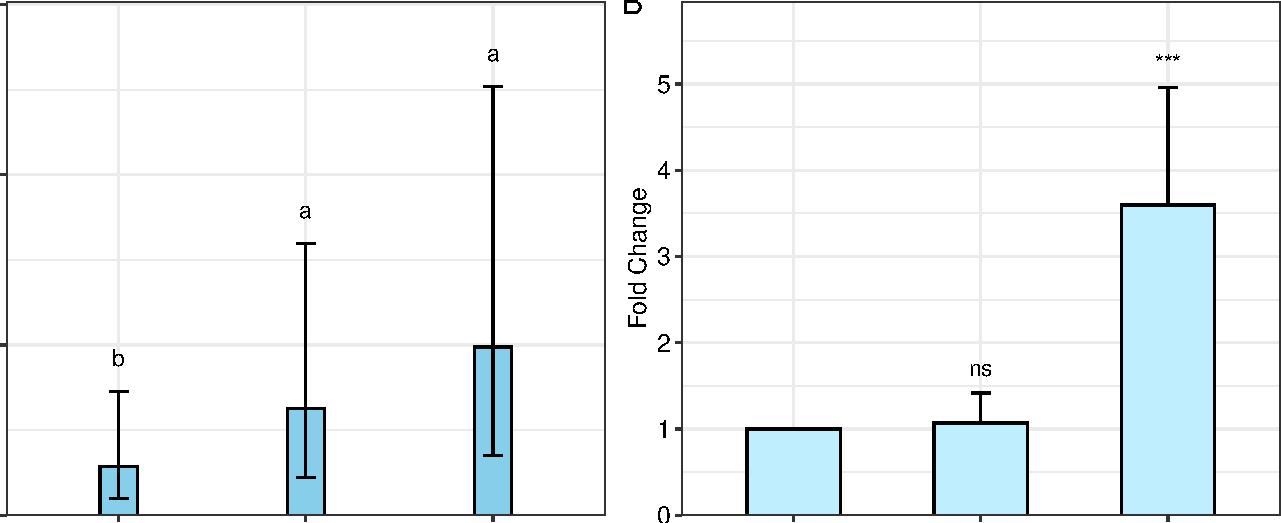
\includegraphics{vignette_files/figure-latex/unnamed-chunk-11-1} 

}

\caption{A) A bar plot representing Relative expression of a gene under three levels of a factor generated using ‘oneFACTORplot’ function, B) Plot of average Fold changes produced by the ‘qpcrANCOVA’ function from the same data as ‘C’. Check level can be changed by user. Error bars represent 95\% confidence interval.}\label{fig:unnamed-chunk-11}
\end{figure}

\hypertarget{barplot-with-the-1-alpha-confidence-interval-as-error-bars}{%
\subsubsection{Barplot with the (1-alpha)\% confidence interval as error
bars}\label{barplot-with-the-1-alpha-confidence-interval-as-error-bars}}

\begin{Shaded}
\begin{Highlighting}[]
\CommentTok{\# Before plotting, the result needs to be extracted as below:}
\NormalTok{res }\OtherTok{\textless{}{-}} \FunctionTok{qpcrANOVA}\NormalTok{(data\_2factor, }\AttributeTok{numberOfrefGenes =} \DecValTok{1}\NormalTok{)}

\CommentTok{\# Plot of the \textquotesingle{}res\textquotesingle{} data with \textquotesingle{}Genotype\textquotesingle{} as grouping factor}
\NormalTok{q1 }\OtherTok{\textless{}{-}} \FunctionTok{twoFACTORplot}\NormalTok{(res,}
   \AttributeTok{x.axis.factor =}\NormalTok{ Drought,}
   \AttributeTok{group.factor =}\NormalTok{ Genotype,}
   \AttributeTok{width =} \FloatTok{0.5}\NormalTok{,}
   \AttributeTok{fill =} \StringTok{"Greens"}\NormalTok{,}
   \AttributeTok{y.axis.adjust =} \FloatTok{0.5}\NormalTok{,}
   \AttributeTok{y.axis.by =} \DecValTok{2}\NormalTok{,}
   \AttributeTok{ylab =} \StringTok{"Relative Expression"}\NormalTok{,}
   \AttributeTok{xlab =} \StringTok{"Drought Levels"}\NormalTok{,}
   \AttributeTok{legend.position =} \FunctionTok{c}\NormalTok{(}\FloatTok{0.15}\NormalTok{, }\FloatTok{0.8}\NormalTok{),}
   \AttributeTok{show.letters =} \ConstantTok{TRUE}\NormalTok{,}
   \AttributeTok{fontsizePvalue =} \DecValTok{4}\NormalTok{)}

\CommentTok{\# Plotting the same data with \textquotesingle{}Drought\textquotesingle{} as grouping factor}
\NormalTok{q2 }\OtherTok{\textless{}{-}} \FunctionTok{twoFACTORplot}\NormalTok{(res,}
   \AttributeTok{x.axis.factor =}\NormalTok{ Genotype,}
   \AttributeTok{group.factor =}\NormalTok{ Drought,}
   \AttributeTok{xlab =} \StringTok{"Genotype"}\NormalTok{,}
   \AttributeTok{fill =} \StringTok{"Blues"}\NormalTok{,}
   \AttributeTok{legend.position =} \FunctionTok{c}\NormalTok{(}\FloatTok{0.15}\NormalTok{, }\FloatTok{0.8}\NormalTok{),}
   \AttributeTok{show.letters =} \ConstantTok{FALSE}\NormalTok{,}
   \AttributeTok{show.errorbars =}\NormalTok{ F,}
   \AttributeTok{show.points =}\NormalTok{ T,}
   \AttributeTok{fontsizePvalue =} \DecValTok{4}\NormalTok{)}

\FunctionTok{multiplot}\NormalTok{(q1, q2, }\AttributeTok{cols =} \DecValTok{2}\NormalTok{)}
\end{Highlighting}
\end{Shaded}

\begin{verbatim}
## $plot
## 
## $plot
\end{verbatim}

\begin{Shaded}
\begin{Highlighting}[]
\FunctionTok{grid.text}\NormalTok{(}\StringTok{"A"}\NormalTok{, }\AttributeTok{x =} \FloatTok{0.02}\NormalTok{, }\AttributeTok{y =} \DecValTok{1}\NormalTok{, }\AttributeTok{just =} \FunctionTok{c}\NormalTok{(}\StringTok{"right"}\NormalTok{, }\StringTok{"top"}\NormalTok{), }\AttributeTok{gp=}\FunctionTok{gpar}\NormalTok{(}\AttributeTok{fontsize=}\DecValTok{16}\NormalTok{))}
\FunctionTok{grid.text}\NormalTok{(}\StringTok{"B"}\NormalTok{, }\AttributeTok{x =} \FloatTok{0.52}\NormalTok{, }\AttributeTok{y =} \DecValTok{1}\NormalTok{, }\AttributeTok{just =} \FunctionTok{c}\NormalTok{(}\StringTok{"right"}\NormalTok{, }\StringTok{"top"}\NormalTok{), }\AttributeTok{gp=}\FunctionTok{gpar}\NormalTok{(}\AttributeTok{fontsize=}\DecValTok{16}\NormalTok{))}
\end{Highlighting}
\end{Shaded}

\begin{figure}

{\centering 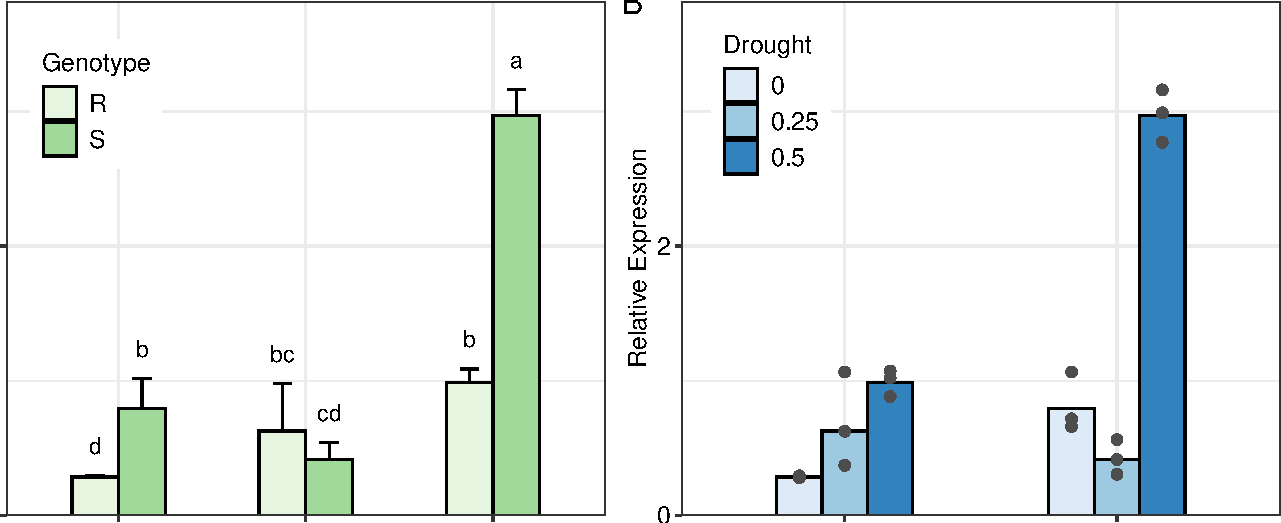
\includegraphics{vignette_files/figure-latex/unnamed-chunk-12-1} 

}

\caption{Average relative expression of a target gene under two different factors of genotype (with two levels) and drought (with three levels). Error bars represent standard deviations. Means (columns) lacking letters in common have significant difference at alpha = 0.05 as resulted from the `LSD.test` of agricolae package.}\label{fig:unnamed-chunk-12}
\end{figure}

\hypertarget{a-three-factorial-experiment-example}{%
\subsubsection{A three-factorial experiment
example}\label{a-three-factorial-experiment-example}}

\begin{Shaded}
\begin{Highlighting}[]
\CommentTok{\# Before plotting, the result needs to be extracted as below:}
\NormalTok{res }\OtherTok{\textless{}{-}} \FunctionTok{qpcrANOVA}\NormalTok{(data\_3factor\_b, }\AttributeTok{numberOfrefGenes =} \DecValTok{1}\NormalTok{)}\SpecialCharTok{$}\NormalTok{Result}
\NormalTok{res}
\end{Highlighting}
\end{Shaded}

\begin{verbatim}
##        Type Conc SA     RE    LCL    UCL letters    std
## R:H:A1    R    H A1 0.9885 1.5455 0.6323      cd 0.0979
## R:H:A2    R    H A2 1.7371 2.7159 1.1110      bc 0.1747
## R:L:A1    R    L A1 0.2852 0.4459 0.1824       f 0.0072
## R:L:A2    R    L A2 0.0641 0.1002 0.0410       g 0.0773
## R:M:A1    R    M A1 0.6271 0.9804 0.4011      de 0.3508
## R:M:A2    R    M A2 0.3150 0.4925 0.2015       f 0.1105
## S:H:A1    S    H A1 2.9690 4.6420 1.8990      ab 0.1955
## S:H:A2    S    H A2 5.1934 8.1197 3.3217       a 0.7893
## S:L:A1    S    L A1 0.7955 1.2438 0.5088       d 0.2190
## S:L:A2    S    L A2 1.5333 2.3973 0.9807       c 0.1562
## S:M:A1    S    M A1 0.4147 0.6483 0.2652      ef 0.1289
## S:M:A2    S    M A2 0.7955 1.2438 0.5088       d 0.2368
\end{verbatim}

\begin{Shaded}
\begin{Highlighting}[]
\CommentTok{\# releveling a factor levels first}
\NormalTok{res}\SpecialCharTok{$}\NormalTok{Conc }\OtherTok{\textless{}{-}} \FunctionTok{factor}\NormalTok{(res}\SpecialCharTok{$}\NormalTok{Conc, }\AttributeTok{levels =} \FunctionTok{c}\NormalTok{(}\StringTok{"L"}\NormalTok{,}\StringTok{"M"}\NormalTok{,}\StringTok{"H"}\NormalTok{))}
\NormalTok{res}\SpecialCharTok{$}\NormalTok{Type }\OtherTok{\textless{}{-}} \FunctionTok{factor}\NormalTok{(res}\SpecialCharTok{$}\NormalTok{Type, }\AttributeTok{levels =} \FunctionTok{c}\NormalTok{(}\StringTok{"S"}\NormalTok{,}\StringTok{"R"}\NormalTok{))}

\CommentTok{\# Arrange the first three colunms of the result table.}
\CommentTok{\# This determines the columns order and shapes the plot output.}
\NormalTok{p1 }\OtherTok{\textless{}{-}} \FunctionTok{threeFACTORplot}\NormalTok{(res,}
    \AttributeTok{arrangement =} \FunctionTok{c}\NormalTok{(}\DecValTok{3}\NormalTok{, }\DecValTok{1}\NormalTok{, }\DecValTok{2}\NormalTok{),}
    \AttributeTok{legend.position =} \FunctionTok{c}\NormalTok{(}\FloatTok{0.2}\NormalTok{, }\FloatTok{0.85}\NormalTok{),}
    \AttributeTok{xlab =} \StringTok{"condition"}\NormalTok{,}
    \AttributeTok{fontsizePvalue =} \DecValTok{4}\NormalTok{)}


\CommentTok{\# When using ci as error, increase y.axis.adjust to see the plot correctly!}
\NormalTok{p2 }\OtherTok{\textless{}{-}} \FunctionTok{threeFACTORplot}\NormalTok{(res,}
   \AttributeTok{arrangement =} \FunctionTok{c}\NormalTok{(}\DecValTok{2}\NormalTok{, }\DecValTok{3}\NormalTok{, }\DecValTok{1}\NormalTok{),}
   \AttributeTok{bar.width =} \FloatTok{0.8}\NormalTok{,}
   \AttributeTok{fill =} \StringTok{"Greens"}\NormalTok{,}
   \AttributeTok{xlab =} \StringTok{"Drought"}\NormalTok{,}
   \AttributeTok{ylab =} \StringTok{"Relative Expression"}\NormalTok{,}
   \AttributeTok{errorbar =} \StringTok{"ci"}\NormalTok{,}
   \AttributeTok{y.axis.adjust =} \DecValTok{8}\NormalTok{,}
   \AttributeTok{y.axis.by =} \DecValTok{2}\NormalTok{,}
   \AttributeTok{letter.position.adjust =} \FloatTok{0.6}\NormalTok{,}
   \AttributeTok{legend.title =} \StringTok{"Genotype"}\NormalTok{,}
   \AttributeTok{fontsize =} \DecValTok{12}\NormalTok{,}
   \AttributeTok{legend.position =} \FunctionTok{c}\NormalTok{(}\FloatTok{0.2}\NormalTok{, }\FloatTok{0.8}\NormalTok{),}
   \AttributeTok{show.letters =} \ConstantTok{TRUE}\NormalTok{,}
   \AttributeTok{fontsizePvalue =} \DecValTok{4}\NormalTok{)}

\FunctionTok{multiplot}\NormalTok{(p1, p2, }\AttributeTok{cols =} \DecValTok{2}\NormalTok{)}
\end{Highlighting}
\end{Shaded}

\begin{verbatim}
## $plot
## 
## $plot
\end{verbatim}

\begin{Shaded}
\begin{Highlighting}[]
\FunctionTok{grid.text}\NormalTok{(}\StringTok{"A"}\NormalTok{, }\AttributeTok{x =} \FloatTok{0.02}\NormalTok{, }\AttributeTok{y =} \DecValTok{1}\NormalTok{, }\AttributeTok{just =} \FunctionTok{c}\NormalTok{(}\StringTok{"right"}\NormalTok{, }\StringTok{"top"}\NormalTok{), }\AttributeTok{gp=}\FunctionTok{gpar}\NormalTok{(}\AttributeTok{fontsize=}\DecValTok{16}\NormalTok{))}
\FunctionTok{grid.text}\NormalTok{(}\StringTok{"B"}\NormalTok{, }\AttributeTok{x =} \FloatTok{0.52}\NormalTok{, }\AttributeTok{y =} \DecValTok{1}\NormalTok{, }\AttributeTok{just =} \FunctionTok{c}\NormalTok{(}\StringTok{"right"}\NormalTok{, }\StringTok{"top"}\NormalTok{), }\AttributeTok{gp=}\FunctionTok{gpar}\NormalTok{(}\AttributeTok{fontsize=}\DecValTok{16}\NormalTok{))}
\end{Highlighting}
\end{Shaded}

\begin{figure}

{\centering 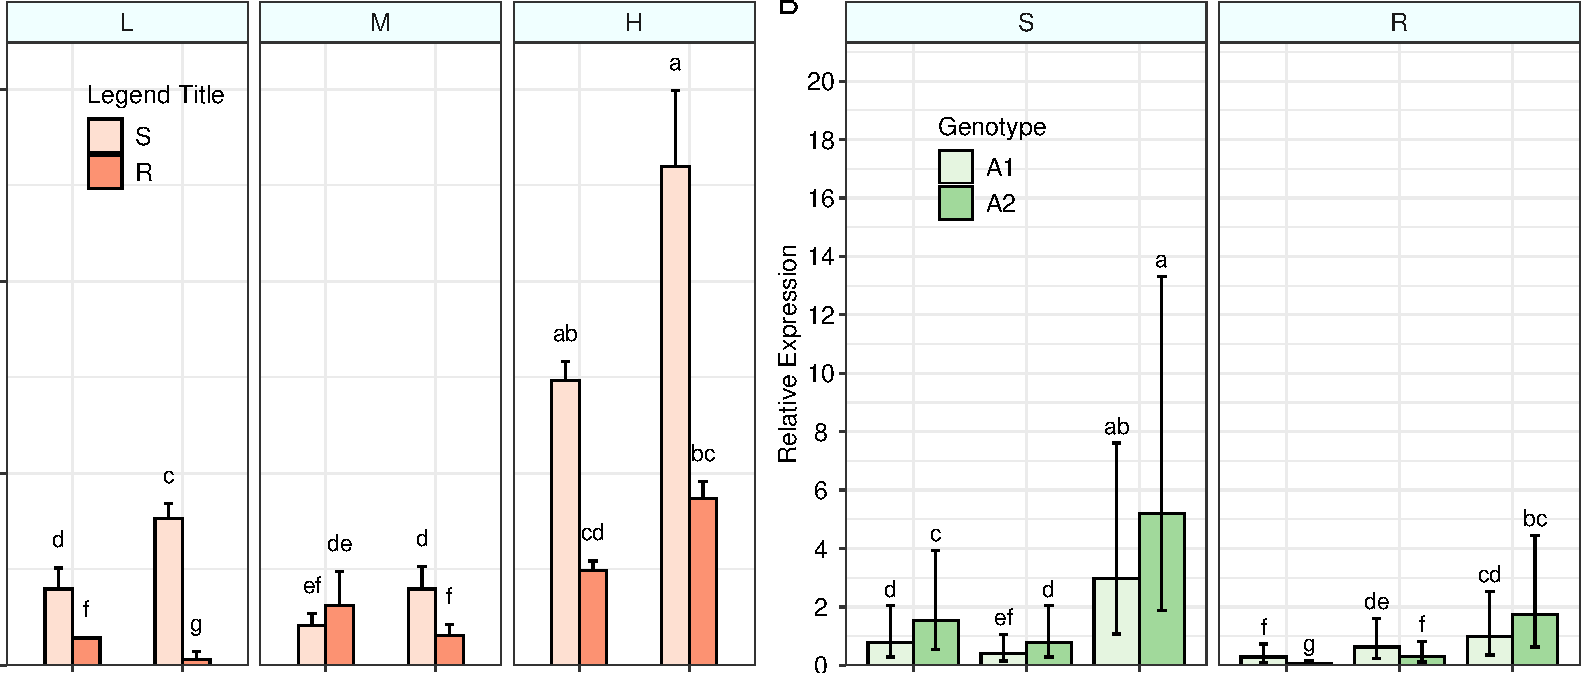
\includegraphics{vignette_files/figure-latex/unnamed-chunk-13-1} 

}

\caption{A and B) Relative expression (RE) of a target gene under two or three factors produced by ‘twoFACTORplot’ and ‘threeFACTORplot’ functions, respectively. Error bars represent standard deviations (can be set to confidence interval). Means (columns) lacking letters in common have significant differences at alpha = 0.05 as resulted from an ‘LSD.test’.}\label{fig:unnamed-chunk-13}
\end{figure}

\hypertarget{an-example-of-showing-point-on-the-plot}{%
\section{An example of Showing point on the
plot}\label{an-example-of-showing-point-on-the-plot}}

\begin{Shaded}
\begin{Highlighting}[]
\NormalTok{b }\OtherTok{\textless{}{-}} \FunctionTok{qpcrANOVA}\NormalTok{(data\_3factor\_a, }\AttributeTok{numberOfrefGenes =} \DecValTok{1}\NormalTok{)}\SpecialCharTok{$}\NormalTok{Result}
\NormalTok{a }\OtherTok{\textless{}{-}} \FunctionTok{qpcrANOVA}\NormalTok{(data\_3factor\_a, }\AttributeTok{numberOfrefGenes =} \DecValTok{1}\NormalTok{)}\SpecialCharTok{$}\NormalTok{Final\_data}

\FunctionTok{ggplot}\NormalTok{(b, }\FunctionTok{aes}\NormalTok{(}\AttributeTok{x =}\NormalTok{ Genotype, }\AttributeTok{y =}\NormalTok{ RE, }\AttributeTok{fill =} \FunctionTok{factor}\NormalTok{(Drought))) }\SpecialCharTok{+}
  \FunctionTok{geom\_bar}\NormalTok{(}\AttributeTok{stat =} \StringTok{"identity"}\NormalTok{, }\AttributeTok{position =} \StringTok{"dodge"}\NormalTok{) }\SpecialCharTok{+}
  \FunctionTok{facet\_wrap}\NormalTok{(}\SpecialCharTok{\textasciitilde{}}\NormalTok{ SA) }\SpecialCharTok{+}
  \FunctionTok{scale\_fill\_brewer}\NormalTok{(}\AttributeTok{palette =} \StringTok{"Reds"}\NormalTok{) }\SpecialCharTok{+}
  \FunctionTok{xlab}\NormalTok{(}\StringTok{"Genotype"}\NormalTok{) }\SpecialCharTok{+}
  \FunctionTok{ylab}\NormalTok{(}\StringTok{"Relative Expression"}\NormalTok{) }\SpecialCharTok{+}
  \FunctionTok{geom\_point}\NormalTok{(}\AttributeTok{data =}\NormalTok{ a, }\FunctionTok{aes}\NormalTok{(}\AttributeTok{x =}\NormalTok{ Genotype, }\AttributeTok{y =}\NormalTok{ (}\DecValTok{10}\SpecialCharTok{\^{}}\NormalTok{(}\SpecialCharTok{{-}}\NormalTok{wDCt)), }\AttributeTok{fill =} \FunctionTok{factor}\NormalTok{(Drought)), }
             \AttributeTok{position =} \FunctionTok{position\_dodge}\NormalTok{(}\AttributeTok{width =} \FloatTok{0.9}\NormalTok{), }\AttributeTok{color =} \StringTok{"black"}\NormalTok{) }\SpecialCharTok{+}
  \FunctionTok{ylab}\NormalTok{(}\StringTok{"ylab"}\NormalTok{) }\SpecialCharTok{+}
  \FunctionTok{xlab}\NormalTok{(}\StringTok{"xlab"}\NormalTok{) }\SpecialCharTok{+}
  \FunctionTok{theme\_bw}\NormalTok{() }\SpecialCharTok{+}
  \FunctionTok{theme}\NormalTok{(}\AttributeTok{axis.text.x =} \FunctionTok{element\_text}\NormalTok{(}\AttributeTok{size =} \DecValTok{12}\NormalTok{, }\AttributeTok{color =} \StringTok{"black"}\NormalTok{, }\AttributeTok{angle =} \DecValTok{0}\NormalTok{, }\AttributeTok{hjust =} \FloatTok{0.5}\NormalTok{),}
        \AttributeTok{axis.text.y =} \FunctionTok{element\_text}\NormalTok{(}\AttributeTok{size =} \DecValTok{12}\NormalTok{, }\AttributeTok{color =} \StringTok{"black"}\NormalTok{, }\AttributeTok{angle =} \DecValTok{0}\NormalTok{, }\AttributeTok{hjust =} \FloatTok{0.5}\NormalTok{),}
        \AttributeTok{axis.title  =} \FunctionTok{element\_text}\NormalTok{(}\AttributeTok{size =} \DecValTok{12}\NormalTok{),}
        \AttributeTok{legend.text =} \FunctionTok{element\_text}\NormalTok{(}\AttributeTok{size =} \DecValTok{12}\NormalTok{)) }\SpecialCharTok{+}
  \FunctionTok{theme}\NormalTok{(}\AttributeTok{legend.position  =} \FunctionTok{c}\NormalTok{(}\FloatTok{0.2}\NormalTok{, }\FloatTok{0.7}\NormalTok{)) }\SpecialCharTok{+}
  \FunctionTok{theme}\NormalTok{(}\AttributeTok{legend.title =} \FunctionTok{element\_text}\NormalTok{(}\AttributeTok{size =} \DecValTok{12}\NormalTok{, }\AttributeTok{color =} \StringTok{"black"}\NormalTok{)) }\SpecialCharTok{+}
  \FunctionTok{scale\_y\_continuous}\NormalTok{(}\AttributeTok{breaks =} \FunctionTok{seq}\NormalTok{(}\DecValTok{0}\NormalTok{, }\FunctionTok{max}\NormalTok{(b}\SpecialCharTok{$}\NormalTok{RE) }\SpecialCharTok{+} \FunctionTok{max}\NormalTok{(b}\SpecialCharTok{$}\NormalTok{std) }\SpecialCharTok{+} \FloatTok{0.1}\NormalTok{, }\AttributeTok{by =} \DecValTok{5}\NormalTok{), }
                     \AttributeTok{limits =} \FunctionTok{c}\NormalTok{(}\DecValTok{0}\NormalTok{, }\FunctionTok{max}\NormalTok{(b}\SpecialCharTok{$}\NormalTok{RE) }\SpecialCharTok{+} \FunctionTok{max}\NormalTok{(b}\SpecialCharTok{$}\NormalTok{std) }\SpecialCharTok{+} \FloatTok{0.1}\NormalTok{), }\AttributeTok{expand =} \FunctionTok{c}\NormalTok{(}\DecValTok{0}\NormalTok{, }\DecValTok{0}\NormalTok{)) }
\end{Highlighting}
\end{Shaded}

\hypertarget{checking-normality-of-residuals}{%
\section{Checking normality of
residuals}\label{checking-normality-of-residuals}}

If the residuals from a \texttt{t.test} or a \texttt{lm} object are not
normally distributed, the grouping letters (deduced from the
\texttt{LSD.test}) might be violated. In such cases, one could apply
another data transformation to the wDCt data for ANOVA and mean
comparison purposes or use non-parametric tests such as the Mann-Whitney
test (also known as the Wilcoxon rank-sum test), \texttt{wilcox.test()},
which is an alternative to \texttt{t.test}, or the
\texttt{kruskal.test()} test which alternative to one-way analysis of
variance, to test the difference between medians of the populations
using independent samples. However, the \texttt{t.test} function (along
with the \texttt{qpcrTTEST} function described above) includes the
\texttt{var.equal} argument. When set to \texttt{FALSE}, perform
\texttt{t.test} under the unequal variances hypothesis.

\begin{Shaded}
\begin{Highlighting}[]
\NormalTok{residuals }\OtherTok{\textless{}{-}} \FunctionTok{qpcrANOVA}\NormalTok{(data\_1factor, }\AttributeTok{numberOfrefGenes =} \DecValTok{1}\NormalTok{)}\SpecialCharTok{$}\NormalTok{lmCRD}\SpecialCharTok{$}\NormalTok{residuals}
\FunctionTok{shapiro.test}\NormalTok{(residuals) }
\end{Highlighting}
\end{Shaded}

\begin{verbatim}
## 
##  Shapiro-Wilk normality test
## 
## data:  residuals
## W = 0.84232, p-value = 0.06129
\end{verbatim}

\begin{Shaded}
\begin{Highlighting}[]
\FunctionTok{qqnorm}\NormalTok{(residuals)}
\FunctionTok{qqline}\NormalTok{(residuals, }\AttributeTok{col =} \StringTok{"red"}\NormalTok{)}
\end{Highlighting}
\end{Shaded}

\begin{figure}

{\centering 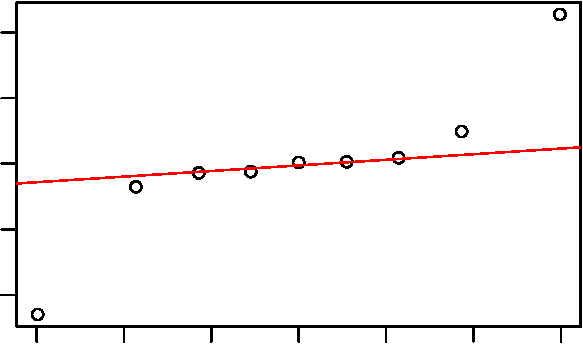
\includegraphics{vignette_files/figure-latex/unnamed-chunk-15-1} 

}

\caption{QQ-plot for the normality assessment of the residuals derived from `t.test` or `lm` functions.}\label{fig:unnamed-chunk-15}
\end{figure}

\hypertarget{mean-of-technical-replicates}{%
\section{Mean of technical
replicates}\label{mean-of-technical-replicates}}

Calculating the mean of technical replicates and getting an output table
appropriate for subsequent ANOVA analysis can be done using the
\texttt{meanTech} function. For this, the input data set should follow
the column arrangement of the following example data. Grouping columns
must be specified under the \texttt{groups} argument of the
\texttt{meanTech} function.

\begin{Shaded}
\begin{Highlighting}[]
\CommentTok{\# See example input data frame:}
\NormalTok{data\_withTechRep}
\end{Highlighting}
\end{Shaded}

\begin{verbatim}
##    factor1 factor2 factor3 biolrep techrep Etarget targetCt Eref  refCt
## 1    Line1    Heat    Ctrl       1       1       2   33.346    2 31.520
## 2    Line1    Heat    Ctrl       1       2       2   28.895    2 29.905
## 3    Line1    Heat    Ctrl       1       3       2   28.893    2 29.454
## 4    Line1    Heat    Ctrl       2       1       2   30.411    2 28.798
## 5    Line1    Heat    Ctrl       2       2       2   33.390    2 31.574
## 6    Line1    Heat    Ctrl       2       3       2   33.211    2 31.326
## 7    Line1    Heat    Ctrl       3       1       2   33.845    2 31.759
## 8    Line1    Heat    Ctrl       3       2       2   33.345    2 31.548
## 9    Line1    Heat    Ctrl       3       3       2   32.500    2 31.477
## 10   Line1    Heat   Treat       1       1       2   33.006    2 31.483
## 11   Line1    Heat   Treat       1       2       2   32.588    2 31.902
## 12   Line1    Heat   Treat       1       3       2   33.370    2 31.196
## 13   Line1    Heat   Treat       2       1       2   36.820    2 31.440
## 14   Line1    Heat   Treat       2       2       2   32.750    2 31.300
## 15   Line1    Heat   Treat       2       3       2   32.450    2 32.597
## 16   Line1    Heat   Treat       3       1       2   35.238    2 31.461
## 17   Line1    Heat   Treat       3       2       2   28.532    2 30.651
## 18   Line1    Heat   Treat       3       3       2   28.285    2 30.745
\end{verbatim}

\begin{Shaded}
\begin{Highlighting}[]
\CommentTok{\# Calculating mean of technical replicates}
\FunctionTok{meanTech}\NormalTok{(data\_withTechRep, }\AttributeTok{groups =} \DecValTok{1}\SpecialCharTok{:}\DecValTok{4}\NormalTok{)}
\end{Highlighting}
\end{Shaded}

\begin{verbatim}
##   factor1 factor2 factor3 biolrep Etarget targetCt Eref    refCt
## 1   Line1    Heat    Ctrl       1       2 30.37800    2 30.29300
## 2   Line1    Heat    Ctrl       2       2 32.33733    2 30.56600
## 3   Line1    Heat    Ctrl       3       2 33.23000    2 31.59467
## 4   Line1    Heat   Treat       1       2 32.98800    2 31.52700
## 5   Line1    Heat   Treat       2       2 34.00667    2 31.77900
## 6   Line1    Heat   Treat       3       2 30.68500    2 30.95233
\end{verbatim}

\hypertarget{citation}{%
\section{Citation}\label{citation}}

\begin{Shaded}
\begin{Highlighting}[]
\FunctionTok{citation}\NormalTok{(}\StringTok{"rtpcr"}\NormalTok{)}
\end{Highlighting}
\end{Shaded}

\hypertarget{contact}{%
\section{Contact}\label{contact}}

Email:
\href{mailto:gh.mirzaghaderi@uok.ac.ir}{\nolinkurl{gh.mirzaghaderi@uok.ac.ir}}

\hypertarget{references}{%
\section{References}\label{references}}

Livak, Kenneth J, and Thomas D Schmittgen. 2001. Analysis of Relative
Gene Expression Data Using Real-Time Quantitative PCR and the Double
Delta CT Method. Methods 25 (4). doi.org/10.1006/meth.2001.1262.

Ganger, MT, Dietz GD, and Ewing SJ. 2017. A common base method for
analysis of qPCR data and the application of simple blocking in qPCR
experiments. BMC bioinformatics 18, 1-11.
doi.org/10.1186/s12859-017-1949-5.

Yuan, Joshua S, Ann Reed, Feng Chen, and Neal Stewart. 2006. Statistical
Analysis of Real-Time PCR Data. BMC Bioinformatics 7 (85).
doi.org/10.1186/1471-2105-7-85.

.

\end{document}
